%!TEX root = ../../master.tex
\section*{Additional Tools and Methods}

In order to get the most possible experience with teaching and speaking publicly, some external presentations have been given. These events have helped us be better instructors and get feedback from the community about what we are trying to accomplish. \\

\noindent The following additional activities have been done during this present master thesis
\begin{itemize}
  \item Docker mentors at 'Docker Meet-up group Aarhus: Docker Birthday 3 years'
  \item Presentation at IT Minds ApS to an internal event
  \item Presentation at Google Developer Group Aarhus meet-up event
  \item Workshop at Praqma about Kubernetes
\end{itemize}
 

\renewcommand*{\arraystretch}{2}
\begin{tabular}{p{6cm}p{7.5cm}}


\includegraphics[align=t,width=6cm]{figures/slides/slides_morgenbooster_itminds} & \textbf{Morgenbooster: Demystifying the cloud} \newline \textit{(39 slides)} \newline 30 minute presentation and demonstration of Microservices, Docker, Kubernetes. Presentation was given at IT Minds ApS, Aarhus, Denmark.  \\ 

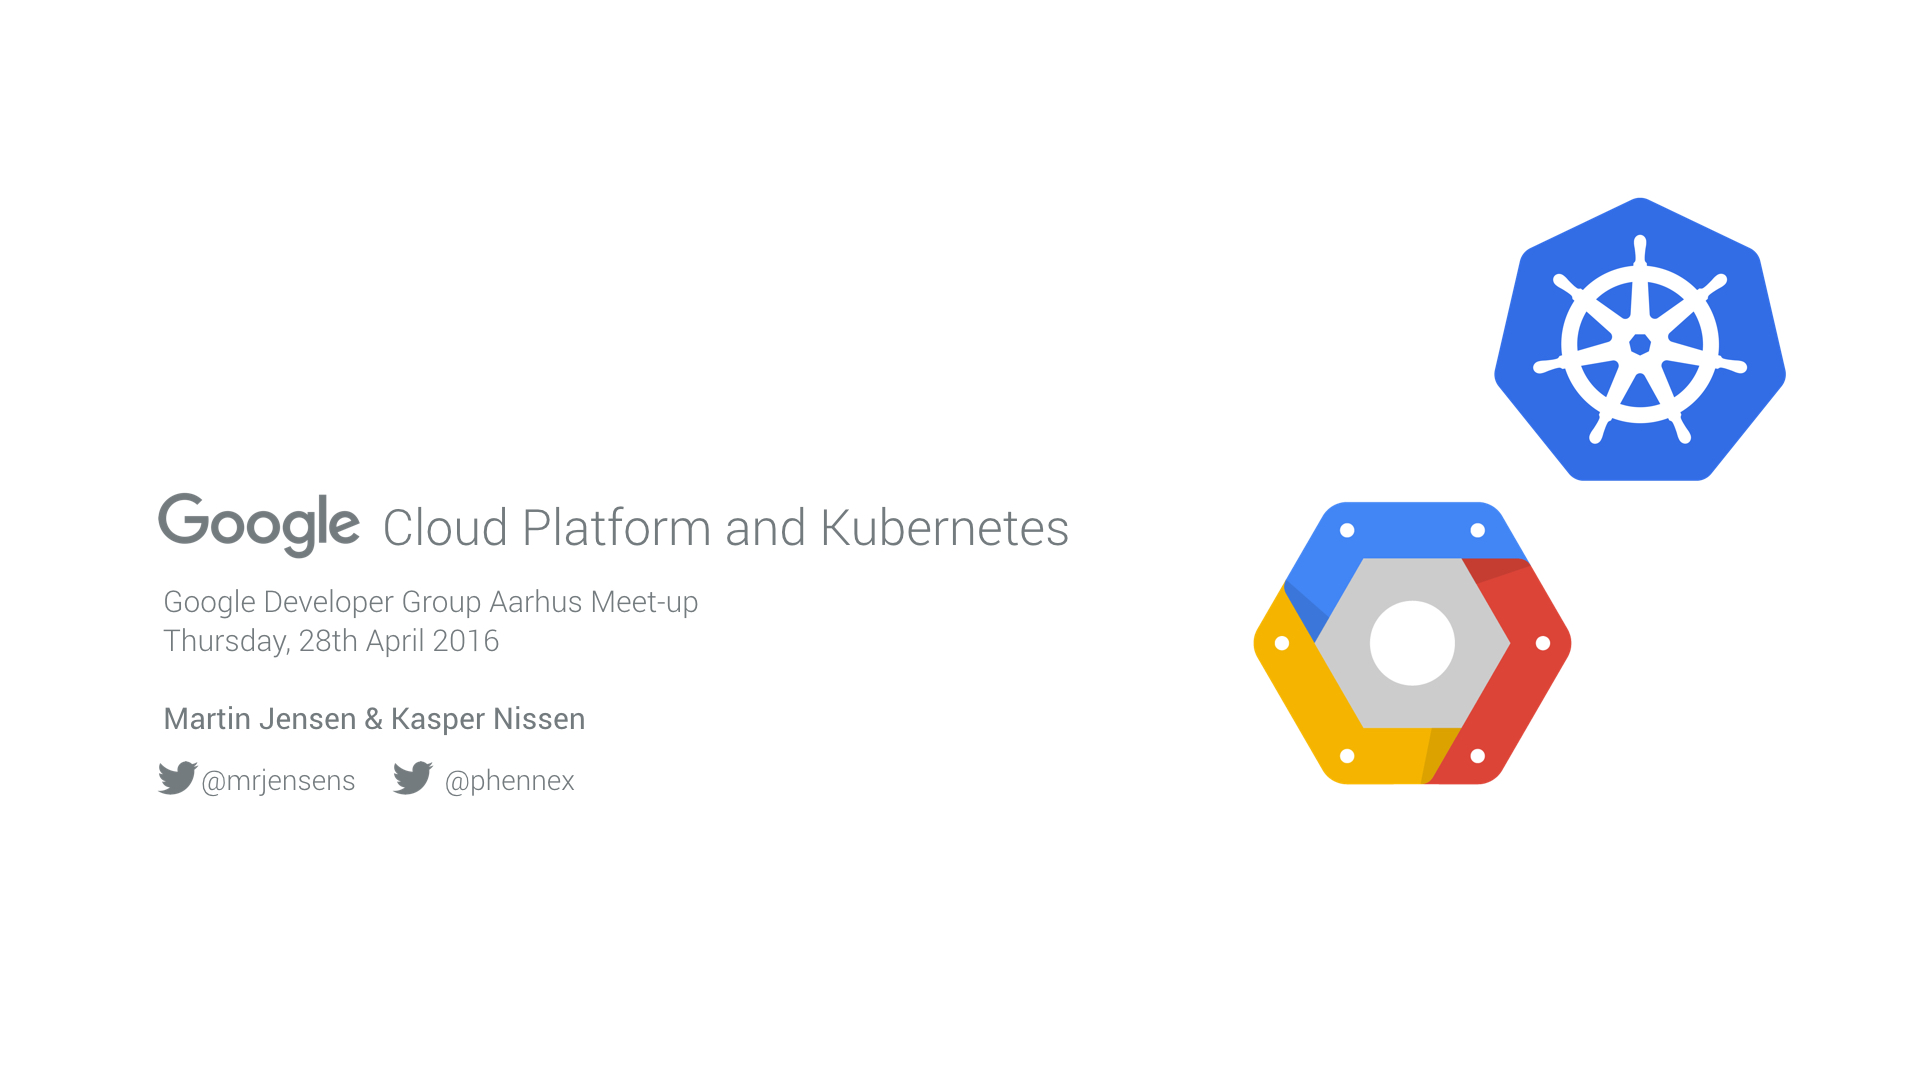
\includegraphics[align=t,width=6cm]{figures/slides/slides_gdg_presentation} & \textbf{Google Developer Group: Google Cloud Platform and Kubernetes} \newline \textit{(93 slides)} \newline 60 minute presentation and demonstration of Cloud Computing, Google Cloud Platform, and Kubernetes. Presentation was given at Google Developer Group Aarhus Meet-up.  \\ 

\end{tabular}
